\chapter*{Proposition 1}
\label{prop:1}

\begin{figure*}[ht]
    \begin{center}
    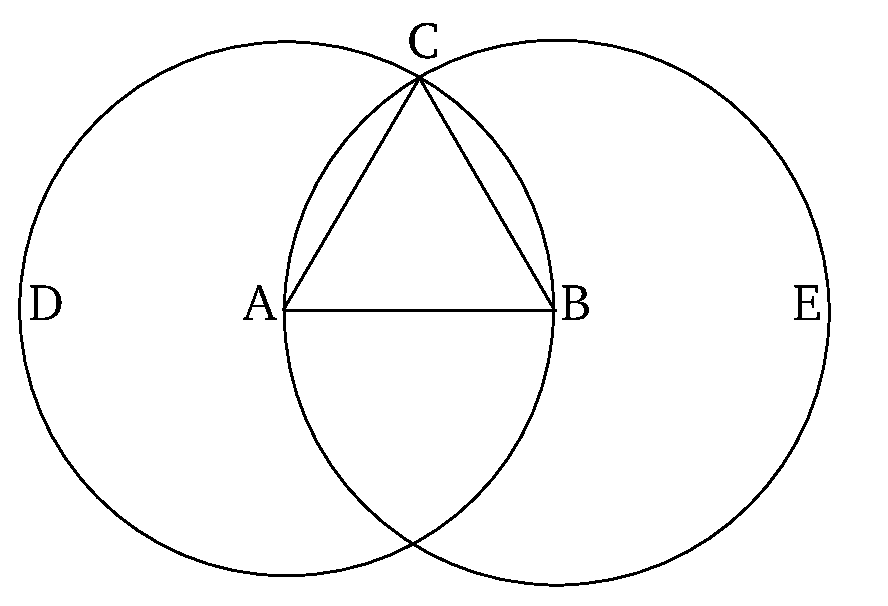
\includegraphics[width=0.5\linewidth]{figures/fig01e.eps}
    \label{fig:prop_1}
    \end{center}
\end{figure*}

To construct an equilateral triangle on a given finite straight-line.

Let $AB$ be the given finite straight-line. 

So it is required to construct an equilateral triangle on the straight-line $AB$.

Let the circle $BCD$ with center $A$ and radius $AB$ have been drawn [Post.~\ref{post:3}], and again let the circle $ACE$ with center $B$ and radius $BA$ have been drawn [Post.~\ref{post:3}].
And let the straight-lines $CA$ and $CB$ have been joined from the point $C$, where the circles cut one another, to the points $A$ and $B$ (respectively) [Post.~\ref{post:1}].

And since the point $A$ is the center of the circle $CDB$, $AC$ is equal to $AB$ [Def.~\ref{def:5}]. Again,
since the point $B$ is the center of the circle $CAE$, $BC$ is equal to $BA$ [Def.~\ref{def:5}]. But $CA$ 
was also shown (to be) equal to $AB$. Thus, $CA$ and $CB$ are each equal to $AB$. But things equal to the same thing are also equal to one another [C.N.~\ref{cn:1}]. Thus, $CA$ is also equal to $CB$. Thus, the three (straight-lines) $CA$, $AB$, and $BC$ are equal to one another.

Thus, the triangle $ABC$ is equilateral, and has been constructed on the
given finite straight-line $AB$. (Which is) the very thing it was required to do.

\section*{Commentary}

\begin{proposition}\label{proposition_1}\lean{Elements.Book1.proposition_1}\leanok
    Given two disctinct points $A$ and $B$ on a line $AB$, there must be a point $C$, s.t. $\triangle~ABC$ is an equilateral triangle.
\end{proposition}
\begin{proof}
    \leanok
    See the original proof by Euclid.
\end{proof}

Euclid omitted the fact that point $C$ can be constructed on either side of $AB$, which is required for proving latter propositions.
We state and prove this fact as Prop.~\ref{proposition_1'}.

\begin{proposition}\label{proposition_1'}\lean{Elements.Book1.proposition_1'}\leanok
    $A$ and $B$ are two disctinct points on a line $AB$. $X$ is a point not on $AB$. Then there must be a point $C$ on the opposite side of $AB$ from $X$, s.t. $\triangle~ABC$ is an equilateral triangle.
\end{proposition}
\begin{proof}
    \leanok
    Similar to Euclid's proof but note that the point $C$ can be constructed on either side.
\end{proof}